\section{System test}
\label{sec:systemtest}

The sections \ref{subsec:tdd} and \ref{subsec:testframe} discussed test-driven development as well as the testing frameworks JSpec and Cucumber. This section will examine how these technologies can be used to create a test suite.

\subsection{Unit tests}
\label{subsec:unittests}

The unit test framework JSpec, which was introduced in section \ref{subsec:jspec}, was used to extensively test the logic contained within business classes and helpers. The tests are distributed over multiple files according to module and functionality. The files contain tests for the following functionality:

\begin{description}
  \item[note\_element\_spec:] Traversing and automatic line storage
  \item[inserting\_note\_element\_spec:] Line insertion
  \item[indenting\_note\_element\_spec:] Line indentation
  \item[unindenting\_note\_element\_spec:] Line outdentation
  \item[focusing\_note\_element\_spec:] Focusing while navigating in the outliner
  \item[rendering\_note\_element\_spec:] Rendering of the tree structure when opening an outline
  \item[outline\_spec, outline\_helpers\_spec:] Outline sorting and rendering
  \item[note\_spec, note\_collection\_spec:] Locating certain lines during the outline rendering process
  \item[resources\_spec:] Abstraction of database interactions
  \item[lib\_spec:] Extensions for the string and array data types
  \item[conflict\_spec:] Display of a line for the resolution of a write conflict
\end{description}
  
The test suite is executed by loading the file {\fontfamily{pcr}\selectfont /\_attachments/spec/index.html} in the browser. The file is documented in listing \ref{code:jspec-index}. It starts by loading the JSpec libraries: the testing framework, the code that needs testing and any other code that is required to run the code that needs testing are loaded. Afterwards it defines the function {\fontfamily{pcr}\selectfont runSuites()}. This function calls the {\fontfamily{pcr}\selectfont exec} method on the {\fontfamily{pcr}\selectfont JSpec} object -which is made available by including the JSpec library- with every of the aforementioned files as its parameter.

Finally, the running of the tests and the output of the results are invoked. This invocation also includes information about the position of the \textit{fixtures}. Fixtures are files that contain HTML blocks. Since the JSpec tests do not run on the database, but merely test the JavaScript functions, a certain DOM state has to be simulated this way. The fixtures are located in the {\fontfamily{pcr}\selectfont /\_attachments/spec/\ fixtures} folder; they contain outlines in multiple states and an HTML representation of the start page. The tests use these HTML pages as the production code would the generated DOM.

The test results are output in the browser. The output may also contain information about failed tests, the number of tests and the time it took to complete them (in figure \ref{fig:jspec-good}, this is just over three seconds).

\medskip
\begin{figure}[ht] 
  \begin{center}
    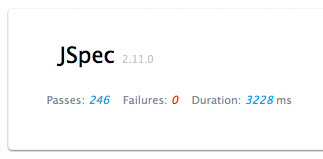
\includegraphics[width=0.5\textwidth]{grafik/jspec-example-good} 
  \end{center}
  \caption{JSpec: Successful completion of all unit tests}
  \label{fig:jspec-good} 
\end{figure}





\subsection{Integration tests}
\label{subsec:integrationtests}

The Cucumber framework was already introduced in section \ref{subsec:cucumber}. It is usually used in combination with the \textit{Webrat} library \cite{webrat:website}. Webrat implements a browser simulator that admittedly does not do JavaScript. Since the application was completely written in JavaScript, the integration tests had to be implemented using a set-up consisting of \textit{HTMLunit} \cite{htmlunit:website}, \textit{Culerity} \cite{culerity:website} and \textit{Celerity} \cite{celerity:website}.

HTMLUnit is a Java library that can parse HTML and execute JavaScript code. HTMLUnit is often regarded as a headless browser \cite{culerity:introduction} since it has the same abilities as a browser, but lacks the user interface in which the pages are displayed. The pages that are read or executed by HTMLUnit can therefore not be seen anywhere. The test suite at hand requires HTMLUnit 2.7 or higher.

Celerity is a JRuby wrapper for HTMLUnit. It has an API for the most common browser functions, which are then executed in HTMLUnit. Culerity is a Ruby gem, which connects Cucumber to Celerity even if the code is not executed in a JRuby environment. When Culerity is used, Celerity starts a Java process to which all Celerity requests are redirected. In the Ruby environment, the results are output as if they were produced by a single Ruby process \cite{culerity:introduction}.

Culerity features a set of common step definitions. These are stored in the folder {\fontfamily{pcr}\selectfont /features\ /step\_definitions/common\_culerity\_steps.rb}. Further step definitions can be found in the same directory.

Section \ref{subsec:cucumber} already specified some examples for features/scenarios (see section \ref{lst:cucumber-feature}) and step definitions (see section \ref{lst:cucumber-steps}). These were taken from the application's test suite. Further features are stored in the {\fontfamily{pcr}\selectfont /features} directory. Figure \ref{fig:cucumber-good} is what it looks like when all scenarios passed successfully. The tests were completed in approximately one and a half minutes. The functions tested were: creation and deletion of an outline; changing the title of an outline; chronological ordering of the outlines in the overview; inserting, editing, indenting and outdenting a line.


\medskip
\begin{figure}[ht] 
  \begin{center}
    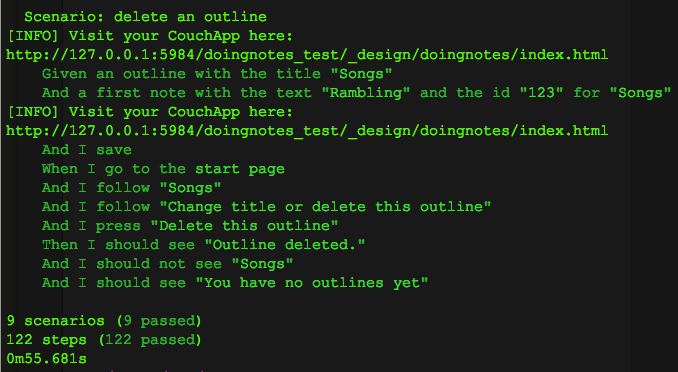
\includegraphics[width=\textwidth]{grafik/cucumber-example-good} 
  \end{center}
  \caption{Cucumber: all tests pass}
  \label{fig:cucumber-good} 
\end{figure}

Culerity does not regard it as a page change if the anchor part of the URL changes. To ensure that it does notify these kind of changes so that Sammy routes may be tested, it is necessary to explicitly execute the route that corresponds to the URL part beyond the anchor. Since this change in Sammy's functionality will deactivate the browser's \enquote{back} function, the behaviour will only be overwritten in the test environment. This is why the test environment is toggled by calling the {\fontfamily{pcr}\selectfont setTestEnv()} function in {\fontfamily{pcr}\selectfont test\_environment.js} using the command \lstinline!$browser.execute_script("setTestEnv();")! for every first step in a scenario. This way, integration tests may be run without impairing the application's behaviour.

\subsection{Test suite for CouchDB's HTTP API}
\label{subsec:testsuite}

The application was developed with the aid of CouchDB's JavaScript HTTP API. This API wraps around basic database functions, which makes formulating database requests easier for developers. Requests can be made as simple JavaScript or jQuery method calls without even having to create an XMLHttpRequest. Since there were no tests available for the API and since some parts of the API were clearly faulty, a test suite was created. It was published under the Apache Licence \cite{jira:testsuite}. Examples taken from the test suite and the API can be found in section \ref{subsec:httpapi}. Additionally, improvements to the API were made \cite{jira:bulkdelete, jira:bulksave}.

Analogous to the test suite for the application, the API tests are executed in the browser. Unlike the aforementioned test suite these tests do access the database, which is why they have to be run by the latter. This means that the files cannot simply be opened in the browser. They have to be located in the {\fontfamily{pcr}\selectfont /share/www} directory of the CouchDB installation and then compiled along with it. The tests can then be accessed by visiting the URL \url{http://localhost:5984/\_utils/spec/run.html}.


\section{Deployment using Amazon Web Services}

The application should not merely be able to \enquote{scale down}, as stipulated in the introduction (section \ref{sec:motivation}, it should also perform well: Even if a large number of users simultaneously synchronise their outlines to the server, this should remain possible without increase in latency. If the CouchDB instance on the server should become temporarily unavailable, the application's availability should still be guaranteed. This can be effortlessly realised using Amazon Web Services.

In the context of prototype development, it was examined how the application might be deployed using the \textit{Amazon Elastic Compute Cloud (EC2)}. Cloud computing's technical background was already discussed in \ref{sec:cloud}. This section will give an overview of the configuration of an application that was deployed using EC2. The overview is supported by own research and \citelit[Chap. 4.1]{cloud:cloudcomputing}.

AWS is an umbrella term for all cloud computing services offered by Amazon. Amazon experiences strong seasonal variation in the demand for its services. Therefore, the majority of these sizable IT resources is not being used for most of the time. The AWS service results from a business idea that makes those free resources available for money, when they are not needed for Amazon's own products.

EC2 allows users to manage virtual servers via Web Services. Such a server is created by following a few steps. These steps are documented by means of screenshots in the appendix (section \ref{subsec:aws}.

A \textit{key pair} is generated after creating an Amazon account. This key pair is used to authenticate the user against the EC2 instance (see fig. \ref{fig:aws-key}). The public key is associated to the Amazon account; the private key stays on the user's computer.

Additionally, a \textit{security group} must be defined and configured (see fig. \ref{fig:aws-group}). Every EC2 instance belongs to such a security group. These groups define the security settings. Individual ports for accessing the server may be opened using the public key generated in the previous step.

The next step involves choosing an \textit{availability zone}, i.e. a geographical region where the server should run. For larger set-ups, distributing over several zones is a way of protecting against the failure of an entire region. It also benefits the latency.

Now, the \textit{amount of resources} required can be defined (see fig. \ref{fig:aws-size}). Several packages are available, varying in processing power, memory and disk space. The packages currently range from 1,7 GB RAM / 160 GB hard disk space to 68,4 GB RAM / 1690 GB hard disk space \cite{aws:instances}.

Finally, an \textit{Amazon Machine Image (AMI)} must be chosen (see fig. \ref{fig:aws-ami}). An AMI is a virtual image, i.e. a snapshot of a virtual server. The different AMIs have varying operating systems and contain different software packages. It is possible to create own images for future (re-)use, and may also be published for a fee. For the testing purpose, however, it suffices to create a virtual server using a ready-made AMI. An up-to-date Ubuntu distribution was chosen, \enquote{alestic's 64bit server Ubuntu 9.04 AMI} with ID \enquote{ami-ccf615a5}.

The EC2 instance is started with the aforementioned parameters. The new virtual server automatically possesses a public IP, under which it can be reached over the Internet, and a private one, which can be used to communicate with other instances. These IPs are re-leased every time the server starts. It is, however, recommendable to set-up an \textit{Elastic IP} (see fig. \ref{fig:aws-ip}). This static ip address can be linked to the server, so the IP address remains the same after every restart.

The instance can normally be managed using the \textit{AWS Management Console} (see fig. \ref{fig:aws-console}). It is available under \url{https://console.aws.amazon.com/ec2/home}. It is also possible to manage the server using the command-line interface; if the public key is saved in {\fontfamily{pcr}\selectfont .ssh/doingnotes.pem}, it is also possible to log in using \lstinline!ssh -i .ssh/doingnotes.pem root@ec2-185-73-233-128.compute-1.amazonaws.com!. As soon as the server is set up, CouchDB can be installed like on a normal Ubuntu computer (see the manual in section \ref{sec:installation}).

As soon as the instance is terminated, all settings and installations that have been made on it will be deleted. In order to make these settings permanent beyond the life cycle of a virtual server, it is necessary to store the instance's state externally. This is where \textit{Amazon Elastic Block Store (EBS)} comes in (see fig. \ref{fig:aws-ebs}). After setting up an EBS it is mounted in the EC2 instance as an external hard disk. It can then be used to store snapshots of the EC2 server.

The price for such an EC2 instance depends on the its performance and is billed by the hour. The price is made up of the amount of resources and data traffic and the amount of time the Elastic IPs and EBS were used. Under \cite{aws:preistabelle}, potential users may calculate the costs of the desired package beforehand.



\section{Clustering with CouchDB Lounge}
\label{subsec:lounge}

This section describes how to distribute the system over several CouchDB instances without changing anything to the user experience. This is where CouchDB Lounge \cite{lounge:website} comes in. CouchDB Lounge is a proxy-based clustering and partitioning application \cite{lounge:SOC}. Both concepts may help to increase a system's availability and performance.

Already in 1997, clustering was suggested as a solution to cope with the increasing needs of modern database applications \citelit{dataplacement}. A computer cluster generally means a number of ...

\begin{quote}
... similar workstations or PCs that are interconnected with a local broadband connection. \citelit[P. 34]{tanenbaum:vs}
\end{quote}

In this very case, clustering means adding redundant CouchDB servers to allow load-balancing and increase availability. Requests are routed to several parallel CouchDB instances. CouchDB also allows redundant storage of data, ensuring that multiple copies of the data are available if the hardware should fail, but this will not be discussed in detail in this thesis.

Horizontal partitioning means dividing the disk space in partitions called \textit{shards}. The shards are distributed over multiple servers in order to increase the throughput to prevent limited hard disk performance from becoming a bottleneck. The next section will discuss this in detail.

\subsection{Functionality}

CouchDB has not been around for long; neither its functionality nor its use have been thoroughly documented. Hence, the following illustration is mainly inspired by \citelit[Chap. 19]{couchdb} and \cite{lounge:wiki}.

Lounge consists of two core modules. A \textit{Smartproxy} deals with CouchDB views and distributes them over the Lounge cluster's nodes. The view performance can be enhanced by increasing the number of nodes in the cluster. The Smartproxy is implemented as a daemon for \textit{Twisted}, a \enquote{framework for writing asynchronous, event-driven networked programs in Python} \cite{twisted}. A \textit{Dumbproxy} is a module for \textit{nginx}, a web server and reverse proxy server. The Dumbproxy is used to handle GET and PUT requests that are not intended for CouchDB views. These requests, too, are distributed over the cluster's individual nodes. The clients are still kept under the impression that their requests are handled by a single CouchDB installation. Both modules use distinct hashes, built by CouchDB Lounge using the documents' IDs. The first characters of these hexadecimal hashes determine the shard to which this document is assigned. The exact assignment is configured in a \textit{shard map}.

Thus, CouchDB Lounge allows creating a cluster that is accessible from the outside under a single address. In figure \ref{fig:lounge-scaling1}, the cluster is depicted as a circle. Two shards are assigned to each of the eight nodes, and each of these shards is identified by a hexadecimal number. If a CouchDB document's ID hash starts with this number, Lounge will save this document in the associated shard. The process then redirects HTTP requests to the actual location of the document. This is how partitioning is implemented.

\medskip
\begin{figure}[H] 
  \begin{center}
    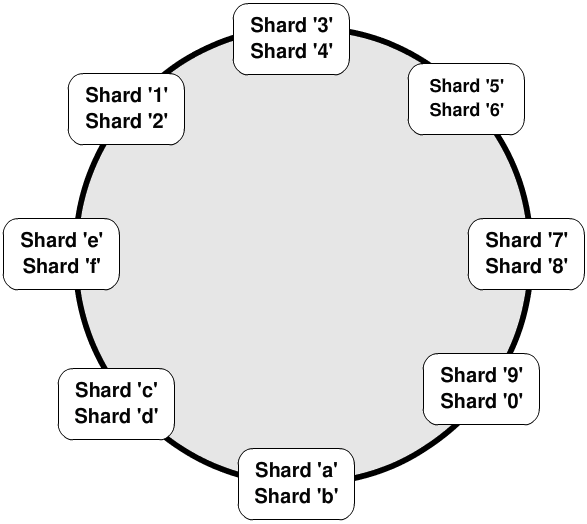
\includegraphics[width=0.6\textwidth]{grafik/shards1} 
  \end{center}
  \caption[16 shards, 8 nodes]{16 shards, 8 nodes. From \citelit{nosql:jan}}
  \label{fig:lounge-scaling1} 
\end{figure}

\begin{quote}
From the outside world, a CouchDB lounge cluster looks just like any other CouchDB node. [...] There's no difference from a functional perspective. [...] Its sharded nature is completely transparent. \cite{lounge:blogpost}
\end{quote}

If the demands for the system's capacity are expected to increase during the system's life cycle, \citelit{couchdb} and \cite{lounge:till} recommend to aim for as many shards as possible in the beginning. The process of distributing the data over more shards than there are nodes is called \enquote{oversharding}. Even if just a few nodes are enough to start with, this amount can later be increased by adding more nodes. The shards are then distributed among these nodes. This is illustrated in \ref{fig:lounge-scaling1}. The system in figure \ref{fig:lounge-scaling1} kept its interface, but the CouchDB instances in the nodes have been replaced by Lounge configurations. If further shards are added afterwards, the entire cluster must be rebuilt.

medskip
\begin{figure}[H] 
  \begin{center}
    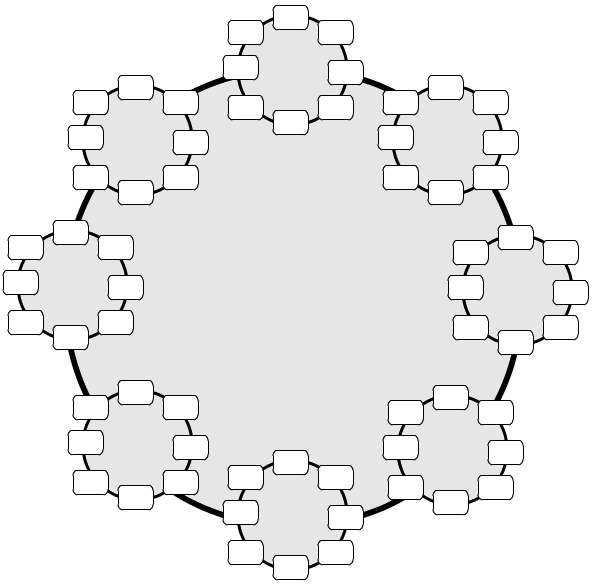
\includegraphics[width=0.6\textwidth]{grafik/shards2} 
  \end{center}
  \caption[16 shards, 8 nodes with 16 subshards, 8 subnodes each]{16 shards, 8 nodes with 16 subshards, 8 subnodes each. From \citelit{nosql:jan}}
  \label{fig:lounge-scaling2} 
\end{figure}

Even for smaller projects, oversharding benefits operation speeds as smaller numbers of documents keep the index size low.

\subsection{Configuration}
\label{subsec:lounge-install}

\cite{lounge:website} contains CouchDB Lounge's source code. It contains instructions for the installation of Dumbproxy, Smartproxy and \textit{Python Lounge}, a collection of required modules. The current version of CouchDB Lounge depends on CouchDB version 0.10.0. The patch that unlocks the required \enquote{design-only replication} exists only for this version. Future versions of CouchDB will come with this feature pre-installed.

\cite{lounge:twoinstances} describes how several CouchDB instances may be installed on a single computer. The central CouchDB configuration file in {\fontfamily{pcr}\selectfont /etc/couchdb/local.ini} must be copied as many times as there are instances. Listing \ref{lst:local.ini} contains the most important parts from its copy in {\fontfamily{pcr}\selectfont local-1.ini}. The copies in {\fontfamily{pcr}\selectfont local-2.ini} etc. contain the corresponding port and log file.
 
\medskip
\begin{lstlisting}[caption=Extract from the CouchDB configuration file, label=lst:local.ini]
[httpd] 
port = 5984
bind_address = 127.0.0.1

[log]
file = /var/log/couchdb/couch-1.log
\end{lstlisting}


Listing \ref{lst:startcouch} shows how to start the first CouchDB instance on a Unix system (Mac OS X 10.6):


\medskip
\begin{lstlisting}[caption=Starting a CouchDB instance, label=lst:startcouch]
sudo -i -u couchdb '/usr/local/bin/couchdb -a etc/couchdb/local-1.ini -p /usr/local/var/run/couchdb/couchdb-1.pid -o /usr/local/var/log/couchdb/error-1.log -e /usr/local/var/log/couchdb/error-1.log -b'
\end{lstlisting}

If the desired number of CouchDB nodes is set up and started, the set-ups are checked for integrity by running the CouchDB test suite as described in the installation manual. If the tests pass successfully, CouchDB Lounge has to be configured before it can be used. This is done by modifying the \url{/var/lounge/etc/shards.conf} file, indicating the number of shards and the level of redundancy. The file contains the JSON object {\fontfamily{pcr}\selectfont nodes} which contains information about the number of CouchDB nodes. Every entry in the array contains the host name and port of an individual node. {\fontfamily{pcr}\selectfont shard\_map} is an array consisting of arrays which defines the location of individual shards and where they should be replicated to. Any number of nodes and any level of redundancy may be specified.

Listing \ref{lst:shardsconf} describes two shards on two nodes. The first shard (number 0) is located on node 0, the second (number 1) on node 1. The first one is replicated to node 1, in case node 0 should fail, and vice-versa.

\lstset{language=bash}
\medskip
\begin{lstlisting}[caption=shards.conf with two nodes and simple redundancy, label=lst:shardsconf]
{
  "shard_map": [[0,1], [1,0]],
  "nodes": [ ["localhost", 5984], ["localhost", 5985] ]
}
\end{lstlisting}

Listing \ref{lst:shardsconf-long} defines a cluster with eight shards, distributed over four nodes with no redundancy. The nodes in both examples are located on the same computer, but they may be distributed over several systems by indicating another host name.

\medskip
\begin{lstlisting}[caption=shards.conf with four nodes and no redundancy and simple oversharding, label=lst:shardsconf-long]
{
  "shard_map": [[0], [1], [2], [3], [0], [1], [2], [3]],
  "nodes": [ ["localhost", 5984], ["localhost", 5985], ["localhost", 5986], ["localhost", 5987]] ]
}
\end{lstlisting}

The installation and configuration of CouchDB has been successful if a document that was created on one node is automatically copied to all the nodes for which redundancy is defined in {\fontfamily{pcr}\selectfont shard\_map}.